% Made up for the tikra benchmark.
\usetikzlibrary{intersections}
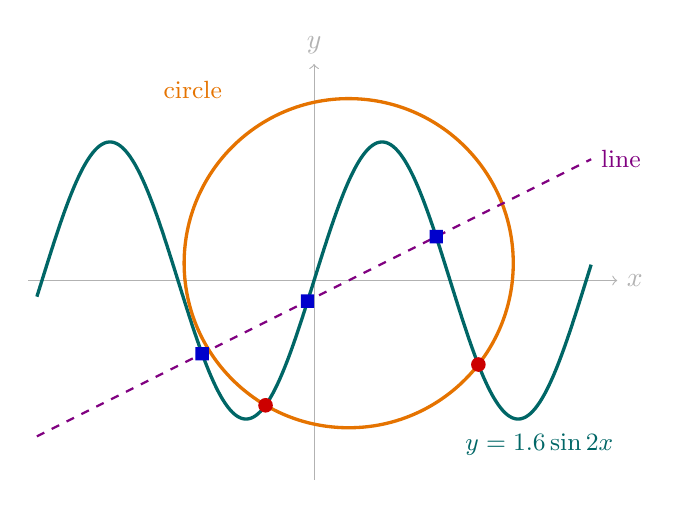
\begin{tikzpicture}[scale=1.1]
  \draw[gray!60, ->] (-3.3,0) -- (3.5,0) node[right] {$x$};
  \draw[gray!60, ->] (0,-2.3) -- (0,2.5) node[above] {$y$};
  \draw[name path=wave, very thick, teal!80!black, domain=-3.2:3.2, samples=120, smooth]
    plot (\x, {1.6*sin(\x*2 r)});
  \draw[name path=ring, very thick, orange!90!black] (0.4,0.2) circle (1.9);
  \draw[name path=line, thick, violet, dashed] (-3.2,-1.8) -- (3.2,1.4);
  \fill[name intersections={of=wave and ring, name=p, total=\t}, red!80!black]
    \foreach \k in {1,...,\t} { (p-\k) circle (2.4pt) };
  \fill[name intersections={of=wave and line, name=q, total=\t}, blue!80!black]
    \foreach \k in {1,...,\t} { (q-\k) +(-2.2pt,-2.2pt) rectangle +(2.2pt,2.2pt) };
  \node[teal!80!black, font=\small] at (2.6,-1.9) {$y = 1.6\sin 2x$};
  \node[orange!90!black, font=\small] at (-1.4,2.2) {circle};
  \node[violet, font=\small, right] at (3.2,1.4) {line};
\end{tikzpicture}
